%% LyX 2.3.6 created this file.  For more info, see http://www.lyx.org/.
%% Do not edit unless you really know what you are doing.
\documentclass[english]{article}
\usepackage[T1]{fontenc}
\usepackage[latin9]{inputenc}
\usepackage{color}
\usepackage{graphicx}

\makeatletter
%%%%%%%%%%%%%%%%%%%%%%%%%%%%%% User specified LaTeX commands.
\usepackage{babel}


\makeatother

\usepackage{babel}
\begin{document}
\title{\texttt{\textbf{CLI Tetris Manual}}}
\author{by JakeTheSillySnake (nettiehu)}
\date{Last updated May 2024}

\maketitle
\tableofcontents{}

\section{Introduction}

This document describes how to install, run, check and remove CLI\footnote{Command Line Interface}
tetris on Mac and Linux systems. Before running, make sure your \textcolor{blue}{gcc}
and \textcolor{blue}{make} packages are up to date (for tests, you'll
also need \textcolor{blue}{gcov} and \textcolor{blue}{lcov} installed;
other \texttt{make} targets, such as \texttt{dist}, \texttt{dvi} and
\texttt{check} use additional utilities\footnote{see \emph{Makefile} for more}).
This program was written on Ubuntu 22.04, so it's possible other systems'
configuration differs slightly.

\section{Installation \& Running}

\subsection{In the beginning...}

Download or clone\footnote{\emph{git clone <link to the repository>} --- note: you'll need GitLab
account access and \textcolor{blue}{git} utility installed} the source repository to where you can easily find it. Then type
and run the following commands in the terminal: 
\begin{enumerate}
\item \texttt{cd <path-to-tetris-folder>/src/gui/cli} 
\item \texttt{make install} 
\item \texttt{make tetris} 
\end{enumerate}
Now the program is installed and compiled, placing all necessary files
in a single folder named \texttt{tetris/}. To start it, run the following: 
\begin{enumerate}
\item \texttt{cd tetris/} 
\item \texttt{./tetris.out} 
\end{enumerate}
If there are errors, you're likely missing some packages. Try to install
everything you need to ensure the program runs smoothly.

\subsection{How to play}

This program is a classic version reimagining. Your task is to make
horizontal lines from randomly generated falling pieces. Each completed
line earns you points, insreasing the level of difficulty and speed.
There are 10 levels and 7 possible pieces. Pay attention to the following
controls: 
\begin{description}
\item [{S}] start 
\item [{Arrow~Left}] move left 
\item [{Arrow~Right}] move right 
\item [{Arrow~Down}] fast fall 
\item [{Shift}] rotate clockwise 
\item [{Space}] pause/resume 
\item [{Q}] quit 
\end{description}

\section{Game structure \& testing}

CLI tetris uses a finite state machine (FSM) to manage the game's
state. The source code can be found in \texttt{tetris/fsm\_table.c}.
It controls switching between 8 states: 
\begin{description}
\item [{Start}] beginning of the game 
\item [{Spawn}] generation of a new piece at the top 
\item [{Shifting}] piece shifts downwards after a set time period 
\item [{Moving}] piece responds to the user's actions 
\item [{Attaching}] piece reaches the bottom or lands on another piece 
\item [{Pause}] the game stops updating the field 
\item [{Gameover}] the game ends when pieces reach the top 
\item [{Exit}] termination of the game 
\end{description}
There is an additional ``secret'' state called FILE\_ERROR, which
closes the game if necessary files can't be accessed. FSM continuously
returns updated game field and stats depending on the user's action.
The relationship between states is depicted below:

%%% Uncomment next life for a diagram. Insert path to the game directory in place of CURRENT_PATH.
%%%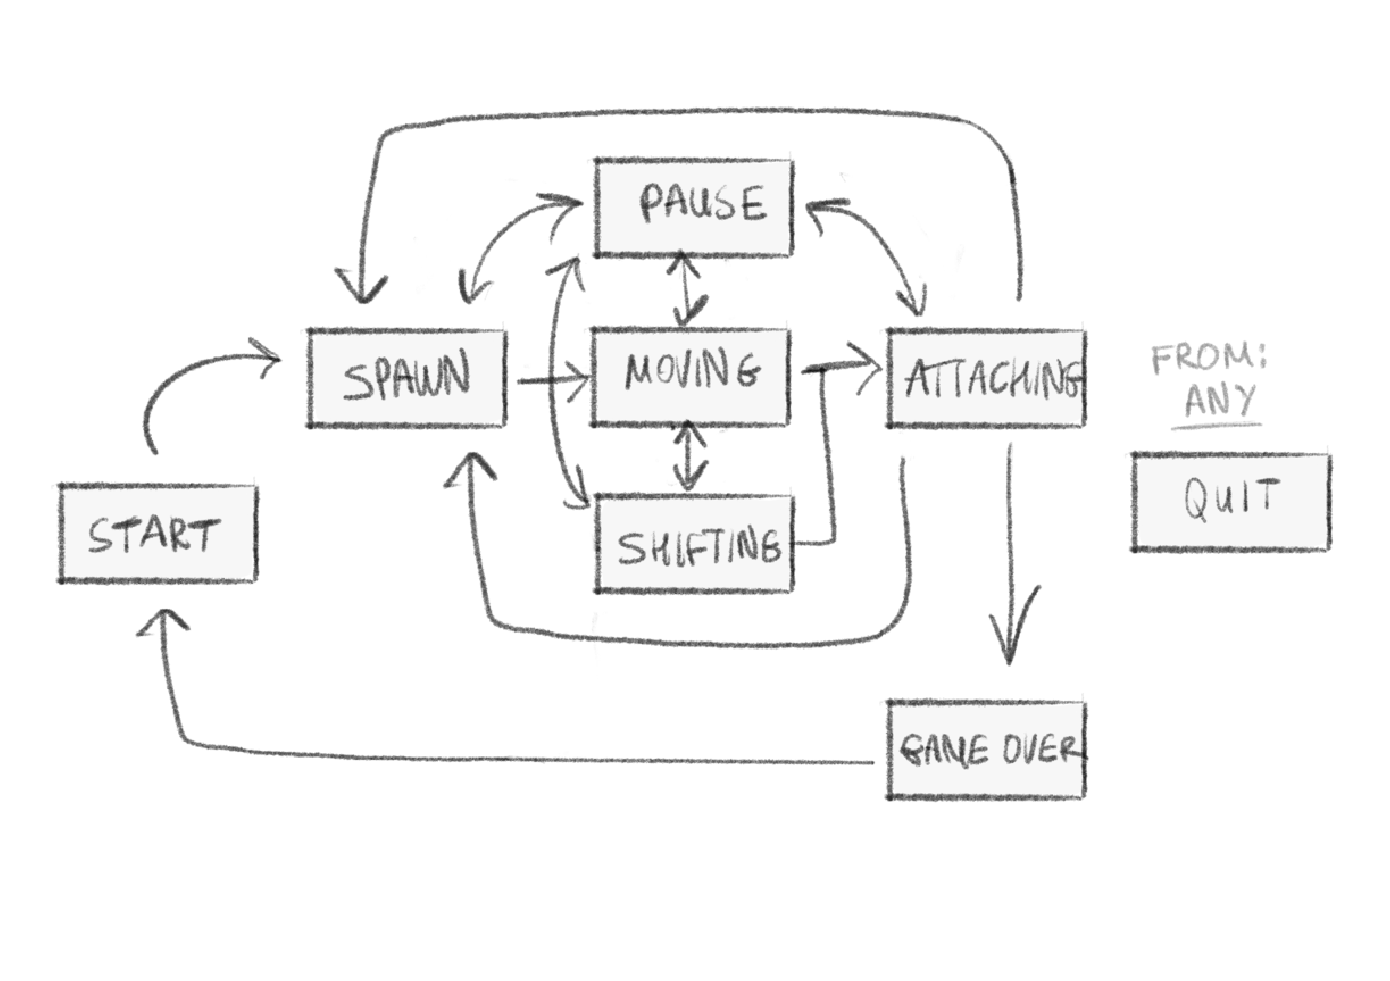
\includegraphics[scale=0.5]{/CURRENT_PATH/C7_BrickGame_v1.0-1/src/brick_game/tetris/assets/fsm_scheme.eps}

The rest of the program is divided between logic (\texttt{tetris/backend.c})
and interface (\texttt{tetris/tetris.c}). The backend file can be
compiled and tested as a library to produce a GCOV report. To do this,
run: 
\begin{enumerate}
\item \texttt{make test} 
\item \texttt{make gcov\_report} 
\end{enumerate}
If you're on Linux, open the \texttt{./report/index.html} file in
a local server for graphic representation. Running \texttt{make} or
\texttt{make all} will reinstall, compile, test the program and produce
the report. You can get DVI documentation with \texttt{make dvi} or
a distribution .tar.gz package with \texttt{make dist}.

\section{Deinstallation}

Simply run \texttt{make uninstall }or\texttt{ make clean. }This will
remove the \texttt{tetris/} directory but not the original download.
I trust you know how to delete the rest.

\subparagraph{If you wish to suggest an improvement or report a bug, contact me
@nettiehu (for School 21).}
\end{document}
